\documentclass[journal,article,submit,moreauthors,pdftex]{Definitions/tsp} 
%%%%Update on 30 November 2023%%%
\usepackage[normalem]{ulem} % For using the command \uuline{} in the \abstract 
\usepackage{amsfonts} % Use for some special math mark
%%\usepackage{pxfonts} % Use for some special math mark 
%\usepackage{wasysym} % Use for some special mark
%\usepackage{subfigure} % For some paper the use \subfigure
\usepackage{mathcomp} % For permille mark
\usepackage{CJKutf8} % For Chinese font
\usepackage{pifont} % For some special mark 
\usepackage{bm} % Forr math enviroment bold format
\usepackage{bbm} % For some math fancy characters
\graphicspath{{./Definitions/}} % Use for import path the figures paper used

\makeatletter
\def\T@n@@nc@d@ngM@cr@M@d{}
\def\LY@n@@nc@d@ngM@cr@M@d{}
\makeatother

\let\orignewcommand\newcommand  % Store the original \newcommand
\let\newcommand\providecommand  % Make \newcommand behave like \providecommand
\usepackage{verse}
\let\newcommand\orignewcommand  % Use the original `\newcommand` in future
\makeatletter
\renewcommand*{\theHpoemline}{\arabic{verse@envctr}.\arabic{poemline}} % Use the original definition from verse.sty
\makeatother

% Define a matrix envrioment
\newsavebox\foobox
\newcommand{\slantbox}[2][.2]{\mbox{%
        \sbox{\foobox}{#2}%
        \hskip\wd\foobox
        \pdfsave
        \pdfsetmatrix{1 0 #1 1}%
        \llap{\usebox{\foobox}}%
        \pdfrestore
}}

%\setlength{\fboxsep}{0cm}

% Define triangledown mark
\let\oldblacktriangledown\blacktriangledown

% Define \dagger using unicode
\renewcommand{\dagger}{\mathchar"2279}
\renewcommand{\ddagger}{\mathchar"227A}

% Define italic In, Max
\newcommand{\mmathit}[1]{
  \ifthenelse{\equal{#1}{\ln}}{\mathit{ln}}{
    \ifthenelse{\equal{#1}{\max}}{\mathit{max}}{\mathit{#1}}
  }
}
\makeatother
\robustify{\footnote}

\DeclareUnicodeCharacter{1E45}{\.{n}}
\DeclareUnicodeCharacter{1E41}{\.{m}}
\DeclareUnicodeCharacter{2003}{\quad}
%\DeclareUnicodeCharacter{0177}{\^{y}}
%\DeclareUnicodeCharacter{101}{\={a}}
\DeclareUnicodeCharacter{2009}{\thinspace}
\DeclareUnicodeCharacter{2002}{\enspace{}}
\DeclareUnicodeCharacter{2005}{\thinspace}
\DeclareUnicodeCharacter{0263}{\textipa{G}}
%\DeclareUnicodeCharacter{117}{\.{e}}
\DeclareUnicodeCharacter{A0}{~}
\DeclareUnicodeCharacter{2460}{\textcircled{\scriptsize{1}}}
\DeclareUnicodeCharacter{2461}{\textcircled{\scriptsize{2}}}
\DeclareUnicodeCharacter{2462}{\textcircled{\scriptsize{3}}}
\DeclareUnicodeCharacter{2463}{\textcircled{\scriptsize{4}}}
\DeclareUnicodeCharacter{2464}{\textcircled{\scriptsize{5}}}
\DeclareUnicodeCharacter{2465}{\textcircled{\scriptsize{6}}}
\DeclareUnicodeCharacter{2466}{\textcircled{\scriptsize{7}}}
\DeclareUnicodeCharacter{2467}{\textcircled{\scriptsize{8}}}
\DeclareUnicodeCharacter{2468}{\textcircled{\scriptsize{9}}}
\DeclareUnicodeCharacter{2070}{\textsuperscript{0}}
\DeclareUnicodeCharacter{2074}{\textsuperscript{4}}
\DeclareUnicodeCharacter{2075}{\textsuperscript{5}}
\DeclareUnicodeCharacter{2076}{\textsuperscript{6}}
\DeclareUnicodeCharacter{2077}{\textsuperscript{7}}
\DeclareUnicodeCharacter{2078}{\textsuperscript{8}}
\DeclareUnicodeCharacter{2079}{\textsuperscript{9}}
\DeclareUnicodeCharacter{02C2}{<}
\DeclareUnicodeCharacter{2033}{\relax\ifmmode '' \else $''$\fi}
\DeclareUnicodeCharacter{2034}{\relax\ifmmode ''' \else $'''$\fi}
\DeclareUnicodeCharacter{2026}{\relax\ifmmode … \else $\ldots$\fi}
\DeclareUnicodeCharacter{0229}{\c{e}}
\DeclareUnicodeCharacter{016F}{\r{u}}
%\DeclareUnicodeCharacter{0218}{\cb{S}}
%\DeclareUnicodeCharacter{0219}{\cb{s}}
%\DeclareUnicodeCharacter{021B}{\cb{t}}
\DeclareUnicodeCharacter{127}{\relax\ifmmode\rm\hbar\else $\rm\hbar$\fi}
\DeclareUnicodeCharacter{3AC}{\relax\ifmmode\acute{\alpha}\else $\acute{\alpha}$\fi}
\DeclareUnicodeCharacter{3AD}{\relax\ifmmode\acute{\varepsilon}\else $\acute{\varepsilon}$\fi}
\DeclareUnicodeCharacter{3AE}{\relax\ifmmode\acute{\eta}\else $\acute{\eta}$\fi}
\DeclareUnicodeCharacter{3AF}{\relax\ifmmode\acute{\iota}\else $\acute{\iota}$\fi}
\DeclareUnicodeCharacter{3CC}{\relax\ifmmode\acute{o}\else $\acute{o}$\fi}
\DeclareUnicodeCharacter{3CD}{\relax\ifmmode\acute{\upsilon}\else $\acute{\upsilon}$\fi}
\DeclareUnicodeCharacter{3CE}{\relax\ifmmode\acute{\omega}\else $\acute{\omega}$\fi}
\DeclareUnicodeCharacter{391}{A}
\DeclareUnicodeCharacter{392}{B}
\DeclareUnicodeCharacter{395}{E}
\DeclareUnicodeCharacter{396}{Z}
\DeclareUnicodeCharacter{397}{H}
\DeclareUnicodeCharacter{399}{I}
\DeclareUnicodeCharacter{39A}{K}
\DeclareUnicodeCharacter{39C}{M}
\DeclareUnicodeCharacter{39D}{N}
\DeclareUnicodeCharacter{39F}{O}
\DeclareUnicodeCharacter{3A1}{P}
\DeclareUnicodeCharacter{3A4}{T}
\DeclareUnicodeCharacter{3A7}{X}

\DeclareUnicodeCharacter{27E6}{\relax\ifmmode \llbracket \else $\llbracket$\fi}
\DeclareUnicodeCharacter{27E7}{\relax\ifmmode \rrbracket \else $\rrbracket$\fi}

\DeclareUnicodeCharacter{1D434}{\relax\ifmmode A \else $A$\fi}
\DeclareUnicodeCharacter{1D435}{\relax\ifmmode B \else $B$\fi}
\DeclareUnicodeCharacter{1D436}{\relax\ifmmode C \else $C$\fi}
\DeclareUnicodeCharacter{1D437}{\relax\ifmmode D \else $D$\fi}
\DeclareUnicodeCharacter{1D438}{\relax\ifmmode E \else $E$\fi}
\DeclareUnicodeCharacter{1D439}{\relax\ifmmode F \else $F$\fi}
\DeclareUnicodeCharacter{1D43A}{\relax\ifmmode G \else $G$\fi}
\DeclareUnicodeCharacter{1D43B}{\relax\ifmmode H \else $H$\fi}
\DeclareUnicodeCharacter{1D43C}{\relax\ifmmode I \else $I$\fi}
\DeclareUnicodeCharacter{1D43D}{\relax\ifmmode J \else $J$\fi}
\DeclareUnicodeCharacter{1D43E}{\relax\ifmmode K \else $K$\fi}
\DeclareUnicodeCharacter{1D43F}{\relax\ifmmode L \else $L$\fi}
\DeclareUnicodeCharacter{1D440}{\relax\ifmmode M \else $M$\fi}
\DeclareUnicodeCharacter{1D441}{\relax\ifmmode N \else $N$\fi}
\DeclareUnicodeCharacter{1D442}{\relax\ifmmode O \else $O$\fi}
\DeclareUnicodeCharacter{1D443}{\relax\ifmmode P \else $P$\fi}
\DeclareUnicodeCharacter{1D444}{\relax\ifmmode Q \else $Q$\fi}
\DeclareUnicodeCharacter{1D445}{\relax\ifmmode R \else $R$\fi}
\DeclareUnicodeCharacter{1D446}{\relax\ifmmode S \else $S$\fi}
\DeclareUnicodeCharacter{1D447}{\relax\ifmmode T \else $T$\fi}
\DeclareUnicodeCharacter{1D448}{\relax\ifmmode U \else $U$\fi}
\DeclareUnicodeCharacter{1D449}{\relax\ifmmode V \else $V$\fi}
\DeclareUnicodeCharacter{1D44A}{\relax\ifmmode W \else $W$\fi}
\DeclareUnicodeCharacter{1D44B}{\relax\ifmmode X \else $X$\fi}
\DeclareUnicodeCharacter{1D44C}{\relax\ifmmode Y \else $Y$\fi}
\DeclareUnicodeCharacter{1D44D}{\relax\ifmmode Z \else $Z$\fi}
\DeclareUnicodeCharacter{1D44E}{\relax\ifmmode a \else $a$\fi}
\DeclareUnicodeCharacter{1D44F}{\relax\ifmmode b \else $b$\fi}
\DeclareUnicodeCharacter{1D450}{\relax\ifmmode c \else $c$\fi}
\DeclareUnicodeCharacter{1D451}{\relax\ifmmode d \else $d$\fi}
\DeclareUnicodeCharacter{1D452}{\relax\ifmmode e \else $e$\fi}
\DeclareUnicodeCharacter{1D453}{\relax\ifmmode f \else $f$\fi}
\DeclareUnicodeCharacter{1D454}{\relax\ifmmode g \else $g$\fi}
\DeclareUnicodeCharacter{1D456}{\relax\ifmmode i \else $i$\fi}
\DeclareUnicodeCharacter{1D457}{\relax\ifmmode j \else $j$\fi}
\DeclareUnicodeCharacter{1D458}{\relax\ifmmode k \else $k$\fi}
\DeclareUnicodeCharacter{1D459}{\relax\ifmmode l \else $l$\fi}
\DeclareUnicodeCharacter{1D45A}{\relax\ifmmode m \else $m$\fi}
\DeclareUnicodeCharacter{1D45B}{\relax\ifmmode n \else $n$\fi}
\DeclareUnicodeCharacter{1D45C}{\relax\ifmmode o \else $o$\fi}
\DeclareUnicodeCharacter{1D45D}{\relax\ifmmode p \else $p$\fi}
\DeclareUnicodeCharacter{1D45E}{\relax\ifmmode q \else $q$\fi}
\DeclareUnicodeCharacter{1D45F}{\relax\ifmmode r \else $r$\fi}
\DeclareUnicodeCharacter{1D460}{\relax\ifmmode s \else $s$\fi}
\DeclareUnicodeCharacter{1D461}{\relax\ifmmode t \else $t$\fi}
\DeclareUnicodeCharacter{1D462}{\relax\ifmmode u \else $u$\fi}
\DeclareUnicodeCharacter{1D463}{\relax\ifmmode v \else $v$\fi}
\DeclareUnicodeCharacter{1D464}{\relax\ifmmode w \else $w$\fi}
\DeclareUnicodeCharacter{1D465}{\relax\ifmmode x \else $x$\fi}
\DeclareUnicodeCharacter{1D466}{\relax\ifmmode y \else $y$\fi}
\DeclareUnicodeCharacter{1D467}{\relax\ifmmode z \else $z$\fi}

\DeclareUnicodeCharacter{1E67}{\.{\v s}}
\DeclareUnicodeCharacter{1E11}{\relax\ifmmode \c{d} \else $\c{d}$\fi}
\DeclareUnicodeCharacter{1ECB}{\relax\ifmmode \d{i} \else $\d{i}$\fi}
\DeclareUnicodeCharacter{1D8D}{\relax\ifmmode \textlhookx \else $\textlhookx$\fi}
\DeclareUnicodeCharacter{104}{\relax\ifmmode \k{A} \else $\k{A}$\fi}
\DeclareUnicodeCharacter{211E}{\relax\ifmmode \textrecipe \else $\textrecipe$\fi}
\DeclareUnicodeCharacter{29D}{\relax\ifmmode \textctj \else $\textctj$\fi}

\DeclareUnicodeCharacter{1E2E}{\'{\"I}}
\DeclareUnicodeCharacter{23F}{\textrts}

\DeclareUnicodeCharacter{2C73}{\varw}

\DeclareUnicodeCharacter{2127}{\mho}

\DeclareUnicodeCharacter{28C}{\textturnv}
\DeclareUnicodeCharacter{252}{\textturnscripta}
\DeclareUnicodeCharacter{259}{\schwa}
\DeclareUnicodeCharacter{25B}{\m{e}}
\DeclareUnicodeCharacter{266}{\m{h}}
\DeclareUnicodeCharacter{127}{\B{h}}
\DeclareUnicodeCharacter{27E}{\textfishhookr}
\DeclareUnicodeCharacter{281}{\textinvscr}


\continuouspages{yes}
\firstpage{1} 
\makeatletter 
\setcounter{page}{\@firstpage} 
\makeatother
\pubvolume{1}
\issuenum{1}
\articlenumber{12345}
\pubyear{2025}
\copyrightyear{2025}
\datereceived{Day Month Year}
\dateaccepted{Day Month Year}
\dateonlinefirst{}
\datepublished{}

\usepackage{amsmath,amssymb,amsfonts}
\usepackage{bm}
\usepackage{graphicx}
\usepackage{xcolor}
%\usepackage[numbers,sort&compress]{natbib}
\usepackage{booktabs}
\usepackage{threeparttable}
\usepackage{algorithm}
\usepackage{algpseudocode}
\usepackage{enumerate}
\usepackage{xurl}
\usepackage{flushend}
\newcommand{\keywordSeparator}{; }

\Title{Title}

\newcommand{\orcidauthorA}{0000-0000-0000-0003}
\newcommand{\orcidauthorB}{0000-0000-0000-0004}
\newcommand{\orcidauthorC}{0000-0000-0000-0005}
\newcommand{\orcidauthorD}{0000-0000-0000-0006}
\newcommand{\orcidauthorE}{0000-0000-0000-0007}

\Author{
	San Zhang\textsuperscript{1,2,3,\#}\orcidA{}, 
	Si Li\textsuperscript{1,2,\#}\orcidB{}, 
	Wu Wang\textsuperscript{1}\orcidC{}, 
	Liu Zhao\textsuperscript{1,*}\orcidD{}, 
	and Qi Sun\textsuperscript{1,*}\orcidE{}
}

\AuthorNames{San Zhang, Si Li, Wu Wang, et al. }

\address{%
	\textsuperscript{1} Department/College/School/Faculty/Institute/... A, University A, City A, Code A, Country A
		
	\textsuperscript{2} Department/College/School/Faculty/Institute/... B, University B, City B, Code B, Country B
	
	\textsuperscript{3} Department/College/School/Faculty/Institute/... C, University C, City C, Code C, Country C
}

\corres{Corresponding Author(s): Liu Zhao and Qi Sun. Email: liuzhao@gmail.com and qisun@gmail.com}

\firstnote{These authors contributed equally to this work} 
\secondnote{}

\abstract{This is a one-paper-multiple-typesetting-styles template. With this template, users can easily switch to different LaTeX typesetting styles while maintaining up-to-date content. For example, in case a paper is unfortunately rejected without being reviewed, users can switch to a better journal or conference immediately or even directly. We hope all papers can be accepted in a suitable and satisfying place. }

\keyword{LaTeX\keywordSeparator Typesetting\keywordSeparator Acceptance}

\begin{document}

%%%%%%%%%%%%%%%%%%%%%%%%%%%%%%%%%%%%%%%
\section{Introduction}
\label{sec:1}

This is the introduction. See links \cite{linkEnglish, linkChinese, linkScript} for more information. This is the introduction. See links \cite{linkEnglish, linkChinese, linkScript} for more information. This is the introduction. See links \cite{linkEnglish, linkChinese, linkScript} for more information. This is the introduction. See links \cite{linkEnglish, linkChinese, linkScript} for more information. This is the introduction. See links \cite{linkEnglish, linkChinese, linkScript} for more information. This is the introduction. See links \cite{linkEnglish, linkChinese, linkScript} for more information. This is the introduction. See links \cite{linkEnglish, linkChinese, linkScript} for more information. This is the introduction. See links \cite{linkEnglish, linkChinese, linkScript} for more information. This is the introduction. See links \cite{linkEnglish, linkChinese, linkScript} for more information. This is the introduction. See links \cite{linkEnglish, linkChinese, linkScript} for more information. 

The remaining sections are structured as follows. Section~\ref{sec:2} is the related work. Section~\ref{sec:3} is the methodology. Section~\ref{sec:4} presents the experiments. Section~\ref{sec:5} presents the experimental results and discussion. Section~\ref{sec:6} is the conclusion, which concludes the whole work. Some possible future research directions are proposed. 
\section{Related Work}
\label{sec:2}

This is the related work. This is the related work. This is the related work. This is the related work. This is the related work. This is the related work. This is the related work. This is the related work. This is the related work. This is the related work. 
\section{Methodology}
\label{sec:3}

This is the methodology. This is the methodology. This is the methodology. This is the methodology. This is the methodology. This is the methodology. This is the methodology. This is the methodology. This is the methodology. This is the methodology. 
\section{Experiments}
\label{sec:4}

These are the experiments. These are the experiments. These are the experiments. These are the experiments. These are the experiments. These are the experiments. These are the experiments. These are the experiments. These are the experiments. These are the experiments. 
\section{Results and Discussion} 
\label{sec:5}

These are the results and discussion. These are the results and discussion. These are the results and discussion. These are the results and discussion. These are the results and discussion. These are the results and discussion. These are the results and discussion. These are the results and discussion. These are the results and discussion. These are the results and discussion. 

\subsection{Experimental results}

An example figure is shown in Fig.~\ref{fig:tree}. 

\begin{figure*}
	\centerline{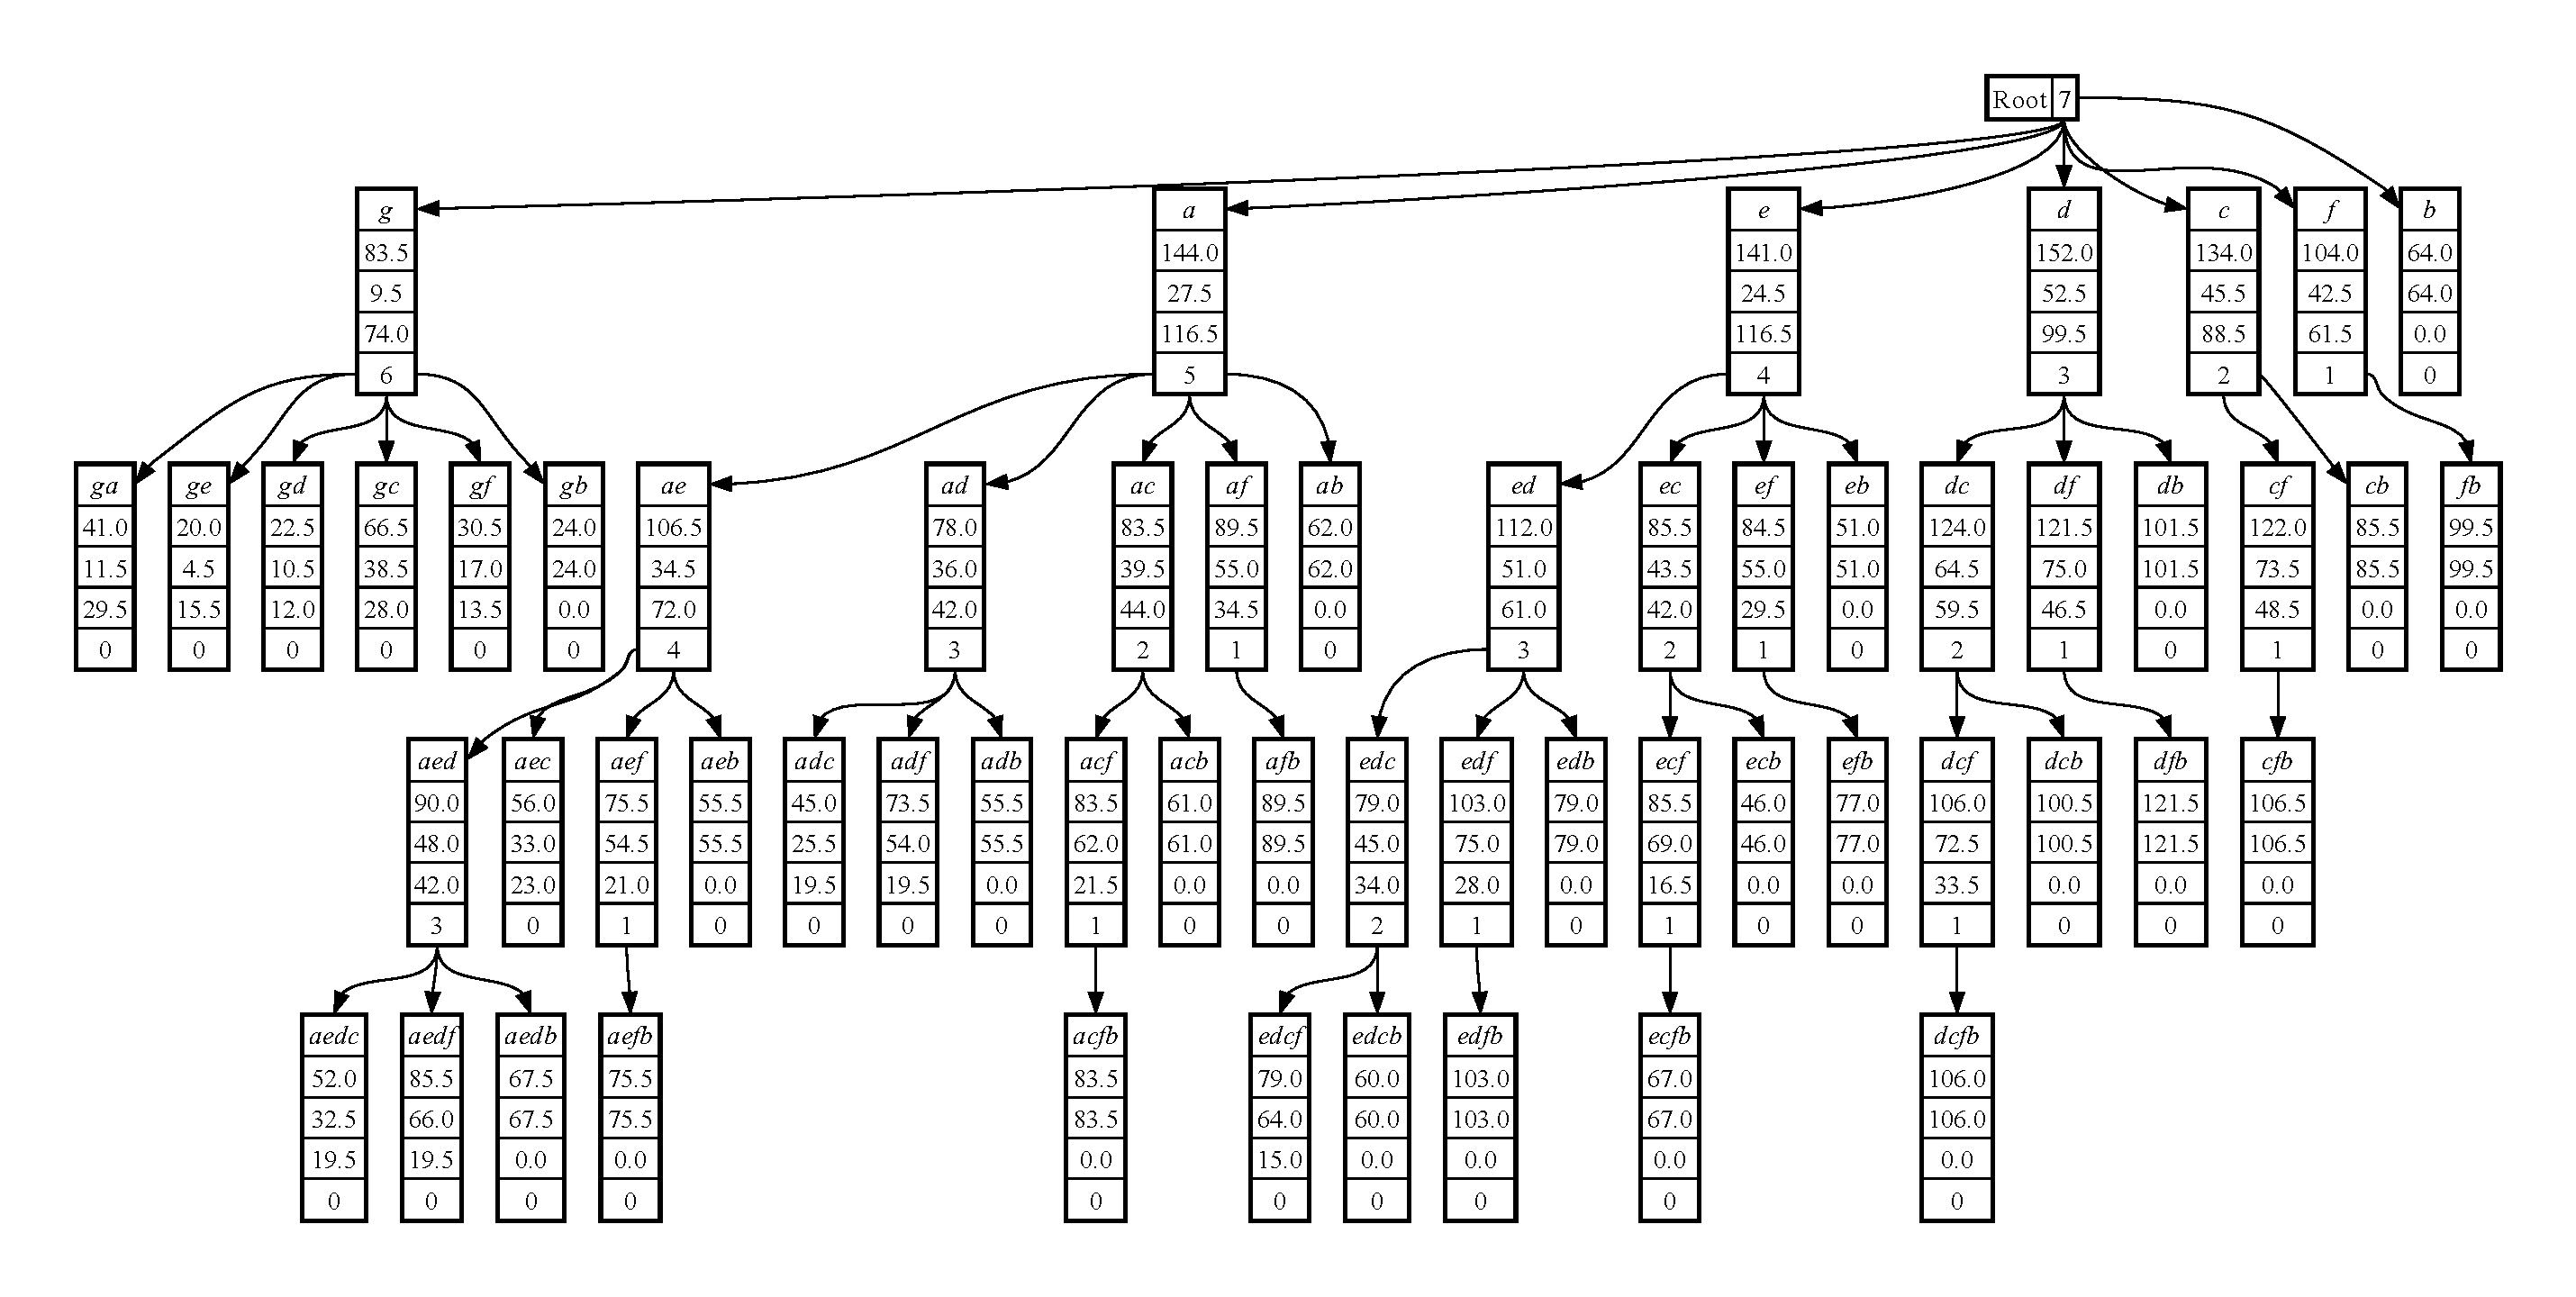
\includegraphics[width=0.95\textwidth]{../Figure/tree.pdf}}
	\caption{This is the tree. }
	\label{fig:tree}
\end{figure*}

\subsection{Discussion}

This is the discussion. This is the discussion. This is the discussion. This is the discussion. This is the discussion. This is the discussion. This is the discussion. This is the discussion. This is the discussion. This is the discussion. 
\section{Conclusion}
\label{sec:6}

This is the conclusion. This is the conclusion. This is the conclusion. This is the conclusion. This is the conclusion. This is the conclusion. This is the conclusion. This is the conclusion. This is the conclusion. This is the conclusion. 

This is the future work. This is the future work. This is the future work. This is the future work. This is the future work. This is the future work. This is the future work. This is the future work. This is the future work. This is the future work. 

\section*{Data Availability}

For the codes and datasets used for accomplishing experiments in this paper, please visit \url{https://github.com/BatchClayderman/onePaperMultipleTypesettingStyles}. 

\section*{Acknowledgement}

Thanks to the editors and the anonymous reviewers for their insightful comments, which improved the quality of this paper. 

\section*{Funding Statement}

There is no funding. 

\section*{Declaration of Competing Interest}

The authors declare that they have no known competing financial interests or personal relationships that could have appeared to influence the work reported in this paper. 

\section*{Authors' Contributions}

All authors reviewed and acknowledged the manuscript. 

\section*{Ethical Consideration Statement}

No human or animal materials are involved in this paper. 
%%%%%%%%%%%%%%%%%%%%%%%%%%%%%%%%%%%%%%%

\reftitle{References}
\bibliography{../Content/ref.bib}

\end{document}  